%%
%% This is file `sample-acmsmall-conf.tex',
%% generated with the docstrip utility.
%%
%% The original source files were:
%%
%% samples.dtx  (with options: `acmsmall-conf')
%% 
%% IMPORTANT NOTICE:
%% 
%% For the copyright see the source file.
%% 
%% Any modified versions of this file must be renamed
%% with new filenames distinct from sample-acmsmall-conf.tex.
%% 
%% For distribution of the original source see the terms
%% for copying and modification in the file samples.dtx.
%% 
%% This generated file may be distributed as long as the
%% original source files, as listed above, are part of the
%% same distribution. (The sources need not necessarily be
%% in the same archive or directory.)
%%
%%
%% Commands for TeXCount
%TC:macro \cite [option:text,text]
%TC:macro \citep [option:text,text]
%TC:macro \citet [option:text,text]
%TC:envir table 0 1
%TC:envir table* 0 1
%TC:envir tabular [ignore] word
%TC:envir displaymath 0 word
%TC:envir math 0 word
%TC:envir comment 0 0
%%
%%
%% The first command in your LaTeX source must be the \documentclass
%% command.
%%
%% For submission and review of your manuscript please change the
%% command to \documentclass[manuscript, screen, review]{acmart}.
%%
%% When submitting camera ready or to TAPS, please change the command
%% to \documentclass[sigconf]{acmart} or whichever template is required
%% for your publication.
%%
%%
\documentclass[acmsmall]{acmart}
\usepackage{todonotes}
%%
%% \BibTeX command to typeset BibTeX logo in the docs
\AtBeginDocument{%
  \providecommand\BibTeX{{%
    Bib\TeX}}}

%% Rights management information.  This information is sent to you
%% when you complete the rights form.  These commands have SAMPLE
%% values in them; it is your responsibility as an author to replace
%% the commands and values with those provided to you when you
%% complete the rights form.
%\setcopyright{acmcopyright}
%\copyrightyear{2018}
%\acmYear{2018}
%\acmDOI{XXXXXXX.XXXXXXX}

%% These commands are for a PROCEEDINGS abstract or paper.
\acmConference[IR'23, Master CS]{}{Spring 2023}{Leiden, the Netherlands}
%%
%%  Uncomment \acmBooktitle if the title of the proceedings is different
%%  from ``Proceedings of ...''!
%%
%%\acmBooktitle{Woodstock '18: ACM Symposium on Neural Gaze Detection,
%%  June 03--05, 2018, Woodstock, NY}

%%
%% For managing citations, it is recommended to use bibliography
%% files in BibTeX format.
%%
%% You can then either use BibTeX with the ACM-Reference-Format style,
%% or BibLaTeX with the acmnumeric or acmauthoryear sytles, that include
%% support for advanced citation of software artefact from the
%% biblatex-software package, also separately available on CTAN.
%%
%% Look at the sample-*-biblatex.tex files for templates showcasing
%% the biblatex styles.
%%

%%
%% The majority of ACM publications use numbered citations and
%% references.  The command \citestyle{authoryear} switches to the
%% "author year" style.
%%
%% If you are preparing content for an event
%% sponsored by ACM SIGGRAPH, you must use the "author year" style of
%% citations and references.
%% Uncommenting
%% the next command will enable that style.
%%\citestyle{acmauthoryear}


%%
%% end of the preamble, start of the body of the document source.
\begin{document}

%%
%% The "title" command has an optional parameter,
%% allowing the author to define a "short title" to be used in page headers.
\title{Final assignment: Cross-encoder re-rankers}

%%
%% The "author" command and its associated commands are used to define
%% the authors and their affiliations.
%% Of note is the shared affiliation of the first two authors, and the
%% "authornote" and "authornotemark" commands
%% used to denote shared contribution to the research.
\author{Siwen Tu}
\author{Shupei Li}
\affiliation{%
  \institution{LIACS, Leiden University}
  \country{the Netherlands}
}

%%
%% By default, the full list of authors will be used in the page
%% headers. Often, this list is too long, and will overlap
%% other information printed in the page headers. This command allows
%% the author to define a more concise list
%% of authors' names for this purpose.
\renewcommand{\shortauthors}{S. Tu and S. Li}

%%
%% The abstract is a short summary of the work to be presented in the
%% article.

%%
%% The code below is generated by the tool at http://dl.acm.org/ccs.cfm.
%% Please copy and paste the code instead of the example below.
%%

%%
%% Keywords. The author(s) should pick words that accurately describe
%% the work being presented. Separate the keywords with commas.
% \keywords{cross-encoder, ensemble methods, information retrieval}

%%
%% This command processes the author and affiliation and title
%% information and builds the first part of the formatted document.
\maketitle

\section{Introduction}
\subsection{Cross-Encoder}
The two-stage retrieval is a common strategy when it comes to retrieving the relevant documents given a query. The first stage is retrieving from the whole document corpus using lexical matching methods such as the BM25 model. The second stage is re-ranking the retrieved documents with a neural model. Cross-encoder is a popular style of model in the second stage of retrieval, which means organizing task inputs (query and candidate texts) into an input template to feed into a transformer for inference, in contrast with the ``bi-encoder'' design where the queries and candidate texts are encoded independently~\cite{lin2020pretrained}. Figure ~\ref{fig:cross-encoder} illustrates the structure of ``cross-encoder". In this task, we explore how to fine-tune and evaluate the cross-encoder re-rankers and how to ensemble different cross-encoder re-rankers using ensemble methods based on the MS Macro dataset. 

\begin{figure}[H]
    \centering
    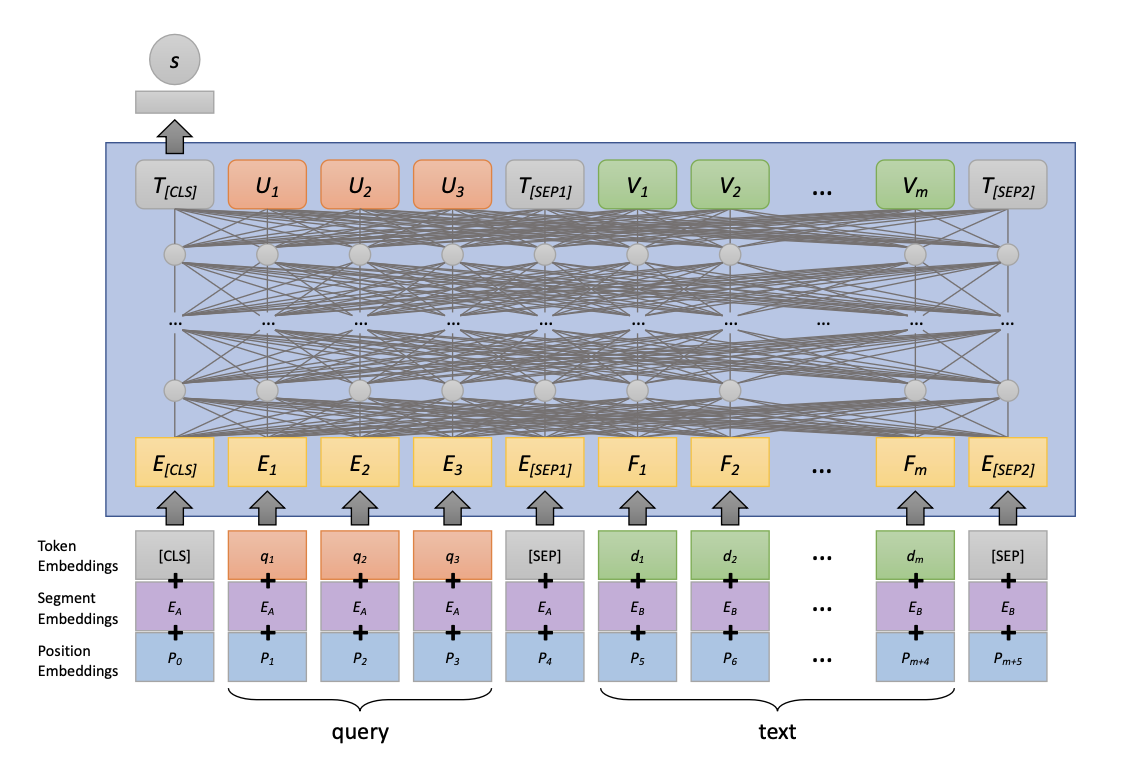
\includegraphics[width=0.7\textwidth]
    {report/cross-encoder.png}
    \caption{Structure of monoBERT Ranking Model, a Two-input Cross-encode re-ranker, Lin et al}
    \label{fig:cross-encoder}
\end{figure}
\subsection{MS Macro Dataset}
We conduct the experiments on the MS Macro dataset. To be more detailed, we fine-tune the cross-encoder models on the MS Macro dataset and evaluate the performance on the TREC 19 DL dataset which is based on the MS Macro dataset. MS Macro is a collection of datasets focused on deep learning in search provided by Microsoft. In this task, we use the passage retrieval dataset containing 8 million passages extracted from web documents retrieved by Bing~\cite{msmarco}. In the fine-tuning phase, the training sample contains $5\times10^6$ query-passage pairs while the development sample contains 200 queries. However, the MS Macro dataset is sparse where usually only one passage is marked as relevant given a query. So in the evaluation phase, we change to the TREC 19 DL dataset,  which is a more dense annotation dataset and suitable for evaluation. In this task, we use 200 queries for evaluation and only consider the queries which have at least one relevant passage.
\section{Task 1: Evaluating cross-encoders}
\begin{table}[!ht]
    \centering
    \caption{Effectiveness results of three fine-tuned cross-encoder models}
    \label{tab:results-task1}
    \begin{tabular}{lllll}
        \toprule
        \textbf{Model} & \textbf{nDCG@10} & \textbf{Recall@100} & \textbf{MAP@1000} & \textbf{\#Training Steps}\\
        \midrule
        MiniLM & 0.674 & 0.495 & 0.433 & 44653 / 156250\\
        TinyBERT & \textbf{0.692} & \textbf{0.508} & \textbf{0.456} & 73999 / 156250\\
        distilroberta & 0.616 & 0.497 & 0.424 & 8999 / 156250\\
        \bottomrule
    \end{tabular}
\end{table}
Table ~\ref{tab:results-task1} shows the results obtained from the fine-tuning and evaluation for three specified cross-encoder models. As we can see from the table ~\ref{tab:results-task1}, the training steps of the three models differ significantly. The overall performance of MiniLM and TinyBERT surpasses that of Distilroberta, which can be attributed to the significant difference in training steps and the fact that the former two models were pre-trained on the MS Macro dataset, unlike the latter. The performance of the MiniLM and TinyBERT is comparable despite the difference in training steps. The reason might be that the difference in architecture compensates for the difference in training steps and the evaluation dataset is suitable for both models. On the other hand, the values of recall@100 for the three models are relatively close, in contrast to the other two metrics. This could be attributed to the fact that recall@100 measures the proportion of relevant passages retrieved among all passages, regardless of the position of the relevant passages. Given that in the MS Macro dataset, the proportion of relevant passages among all passages is small for each query, it is reasonable to expect these three models to perform similarly. 

A higher-performing model is not necessarily more effective for all new, unseen queries. In this task, we train the models on MS Macro dataset and evaluate them on TREC 19 DL dataset. The queries and passages in these two datasets have many common characteristics and structures so the high-performing model tends to perform well during evaluation. However, for new and unseen queries that have different characteristics and distributions from the training dataset, the higher-performing model may not outperform the other models.

As for the limitations of these three models, we can conclude from the results that the training time of these models differs significantly. The training speed of the Distilroberta model is much lower than the other two. So it is essential to take the training time and computational power into account. Besides, these three models are smaller versions of their respective base models. They sacrificed better performance in exchange for effectiveness so they are more suitable for simpler tasks with smaller datasets.
\section{Task 2: Select and apply five ensemble methods}
\begin{table}[!ht]
    \centering
    \caption{Effectiveness results of five ensemble methods}
    \label{tab:results-task2}
    \begin{tabular}{llll}
       \toprule
       \textbf{Model} &  \textbf{nDCG@10} & \textbf{Recall@100} & \textbf{MAP@1000}\\
       \midrule
       Mixed & 0.707 & 0.513 & 0.465\\
       Reciprocal Rank Fusion (RRF) & 0.699 & 0.507 & 0.462\\
       BayesFuse & 0.697 & 0.507 & 0.451\\
       PosFuse & \textbf{0.710} & \textbf{0.516} & \textbf{0.480}\\
       Weighted BordaFuse & 0.707 & 0.511 & 0.464\\
       \bottomrule
    \end{tabular}
\end{table}
Five ensemble methods listed in table ~\ref{tab:results-task2} all require the optimization step and the normalization strategy is min-max. We can conclude from the table ~\ref{tab:results-task2} that the Posfuse model performs best among five models with a outstanding MAP@1000. The values of nDCG@10 and Recall@100 of five models are similar to each other. The Posfuse model is a probability-based method that relies on the probability of a document appearing at a specific position. It is built upon a perfect probability model constructed using the same queries and results for both training and fusion~\cite{DBLP:conf/sigir/LillisZTCLD10}. During the optimization phase of this fusion task, we utilize queries and results from the MS Macro dataset, which is an integral part of the training dataset. This alignment could be the reason why Posfuse outperforms other methods.

In general, the five ensemble models outperform the best single model, TinyBERT, particularly in terms of nDCG@10 and MAP@1000. This outcome confirms that these ensemble methods effectively enhance the retrieval performance of models through their combination. As discussed in task 1, recall@100 measures the proportion of relevant passages retrieved among all passages, without considering the ranked position of the relevant passages. Due to the characteristics of the MS Macro dataset, the improvement of ensemble methods in terms of recall is not as significant when compared to the other two evaluation metrics.

We could use bagging meta-algorithm to ensemble the models. Bagging mainly focus on combining models of low-bias and high-variance and ensemble them to reduce the variance. At the averaging process of bagging, we could aggregate them through assigning different weights to outputs of different models. During the optimization of the fuse methods, they perform a gird search over the search space of hyperparameters. We could using other fine-tuning methods such as genetic algorithm to find the better hyperparameters. Besides, we could use learning to rank method to explore the optimal combination of rankings from different models.
\section{Task 3: Analyzing the most effective ensemble method}
The PosFuse ensemble method in Task 2 outperforms all other methods. Therefore, we apply PosFuse to all combinations of two models out of three in this task and summarize experimental results in Table \ref{tab:results-task3}.
\begin{table}[!ht]
    \centering
    \caption{Effectiveness results of all combinations}
    \label{tab:results-task3}
    \begin{tabular}{llll}
       \toprule
       \textbf{Combination} & \textbf{nDCG@10} & \textbf{Recall@100} & \textbf{MAP@1000}\\
       \midrule
       MiniLM + TinyBERT & \textbf{0.723} & \textbf{0.518} & \textbf{0.483}\\
       MiniLM + distilroberta & 0.691 & 0.509 & 0.463\\
       TinyBERT + distilroberta & 0.694 & 0.507 & 0.468\\
       \bottomrule
    \end{tabular}
\end{table}

MiniLM + TinyBERT ensemble performs best on all metrics. MiniLM + distilroberta performs worst on nDCG@10 and MAP@1000, while TinyBERT + distilroberta performs worst on Recall@100. The result is consistent with our expectations. Because MiniLM and TinyBERT achieve significantly better results than distilroberta in Task 1, we think the performance of the ensemble including distilroberta will be affected by the inferiority of distilroberta. There is no big difference between the performance of MiniLM + distilroberta and that of TinyBERT + distilroberta. However, MiniLM + TinyBERT performs much better than other combinations, which may be caused by removing the distilroberta ranking file. It is worth mentioning that MiniLM + TinyBERT even achieves higher scores than the ensemble of three models in Task 2. This pattern indicates that more models do not mean better performance. A weak model may introduce more noise than information, which impairs the model's performance.

\section{Task 4: Modifying the evaluation metric in fine-tuning}
We modify the CERerankingEvaluator class to change the evaluation metric to nDCG@10. We adopt the implementation in the sklearn package to calculate nDCG@10. Note that the modified class can be easily used by changing the corresponding API in the fine-tuning notebook. No other modification is needed. Our code has been included in the submission.

\section{Task 5: Ensembling through score injection}
In this task, we investigate the effect of the score injection. The score injection is a strategy described in paper \cite{injection} that aims at improving the performance of BERT-based re-rankers by injecting BM25 scores. However, we inject the average scores of MiniLM, TinyBERT, and distilroberta, instead of BM25 scores. Besides, we use the microsoft/MiniLM-L12-H384-uncased model as the re-ranker. Our modified version of the fine-tuning notebook first performs inference with three models and sets the average score as the first sentence of the document. Then the pairs of queries and injected documents are inputted in the re-ranker. Note that we convert the type of the average score into the integer following the suggestion in \cite{injection}. Due to the GPU quota of Colab, we fine-tune the microsoft/MiniLM-L12-H384-uncased model with and without injection for one hour and run the evaluation notebook. The evaluation results are reported in Table \ref{tab:results-task5}. We also include results in \cite{injection} for comparison.
\begin{table}[!ht]
    \centering
    \caption{Effectiveness results of ensembling with and without score injection}
    \label{tab:results-task5}
    \begin{tabular}{llll}
       \toprule
       \textbf{Model} & \textbf{nDCG@10} & \textbf{Recall@100} & \textbf{MAP@1000}\\
       \midrule
       MiniLM-L12-H384-uncased without injection & 0.668 & \textbf{0.503} & 0.450\\
       MiniLM-L12-H384-uncased with injection & 0.664 & 0.495 & 0.435\\
       $\text{MiniLM}_{\text{CAT}}$\cite{injection} & 0.704 & - & 0.452\\
       $\text{MiniLM}_{\text{BM25CAT}}$\cite{injection} & \textbf{0.711} & - & \textbf{0.463}\\
       \bottomrule
    \end{tabular}
\end{table}

MiniLM with BM25 injection has the best performance during evaluation. The performance of MiniLM with the injection of three BERT-based models' predictions does not achieve the anticipated effect. We think one reason is that the training process is not sufficient. Table \ref{tab:results-task5} indicates that our version of MiniLM without injection is not at the expected level as that of $\text{MiniLM}_{\text{CAT}}$. Another reason may be the instability of the model performance. We notice that MiniLM with the average score injection is not very robust during the training. The improvement of the model's robustness is a possible future direction for developing score injection strategies.

%%
%% The next two lines define the bibliography style to be used, and
%% the bibliography file.
\bibliographystyle{ACM-Reference-Format}
\bibliography{main}
%%
%% If your work has an appendix, this is the place to put it.
\end{document}
\endinput
%%
%% End of file `sample-acmsmall-conf.tex'.
